\chapter{Preliminary Results}

\begin{figure}[h]
	\scalebox{0.6}{
	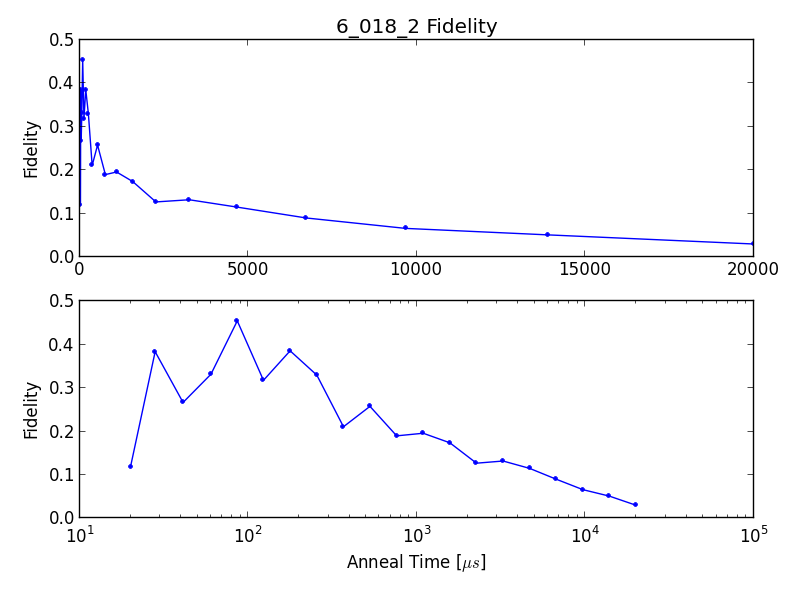
\includegraphics[bb=0 0 800 600]{img/6_018_2_fidelity.png}
}
	\caption[Fidelity vs Time]{Plot of the fidelity as a function of annealing time for the Hamiltonian ``6\_018'' both linear and log-scaled x-axis.}
	\label{fig:fidelity}
\end{figure}

Figure \ref{fig:fidelity} shows the results of 50,000 runs of the annealing machine consisting of 1000 runs at various annealing times.  Along the y-axis is the fidelity, and along the x-axis is the annealing time.  Contrary to what we expect from the adiabatic theorem and simulations of quantum annealing the fidelity is uncorrelated with annealing from 20$\mu$s out to roughly 500$ \mu$s, after which the fidelity \emph{decreases} with increasing annealing time.  This unexpected behaviour leaves us with a number of questions:

\begin{itemize}
	\item For long annealing times, why does the fidelity decrease with increasing annealing times?
	\item For short annealing times, why does the fidelity appear insensitive to annealing time?
	\item Is the short time fidelity dominated by the Hamiltonian programming noise?
	\item Is there significant drift in the fidelities after programming?
	\item Does the Hamiltonian fidelity depend strongly on the number of coupling values?
\end{itemize}

\section{Short Evolution}
\begin{figure}
	\scalebox{0.35}{
		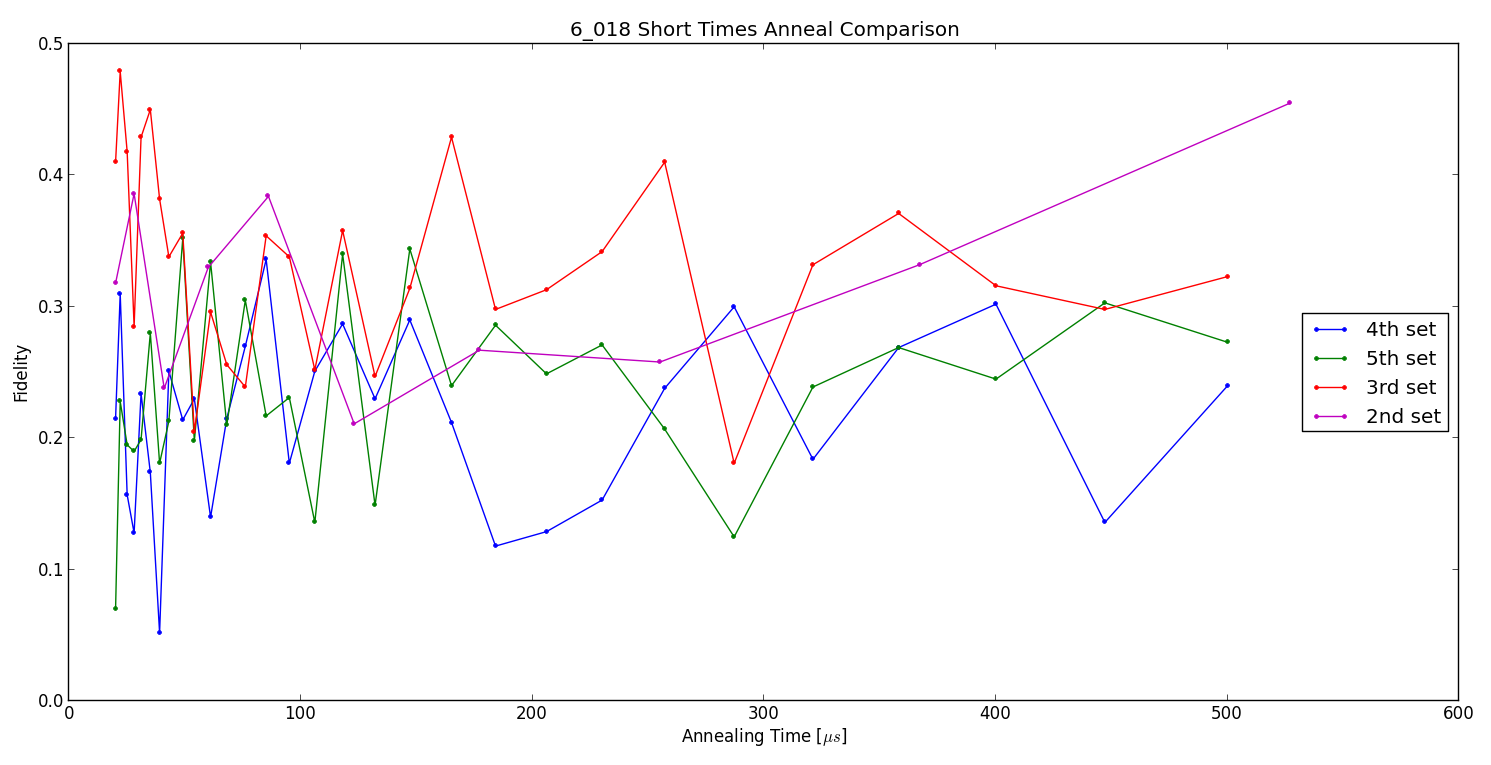
\includegraphics[bb= 0 0 745 382]{img/6_018_comparison.png}
	}
	\caption[Short Time Fidelities]{The fidelity as a function of time for the Hamiltonian ``6\_018'' for several different machine runs.  Each data point consist of 1000 machine reads.  Notice the spread between machine runs is outside of the error bars.}
	\label{fig:short_fidelity}
\end{figure}
As can be seen in Figure \ref{fig:short_fidelity}, there is considerable noise in the fidelities between different machine runs.  The fidelity is determined by computing the fraction of machine reads that return a ground state.  If the assumptions of AQC hold, then the fidelity should depend on only the annealing time.  If this is the case, then we expect that the measured fidelities obey a binomial distribution (think of the machine as being essentially a biased coin, with \texttt{HEADS} being the ground state and \texttt{TAILS} being an excited state).  

To explain this discrepancy we look at a histogram of each fidelity found during the short anneal, Figure \ref{fig:fid_hist}.  Each count in this histogram is a fidelity from a machine run consisting of 1000 machine reads.  This is gently consistent with the noise in the fidelities occurring in the Hamiltonian programming step; that is, the Hamiltonian the machine is evaluating being different from the Hamiltonian we desire.

\begin{figure}
	\scalebox{0.75}{
		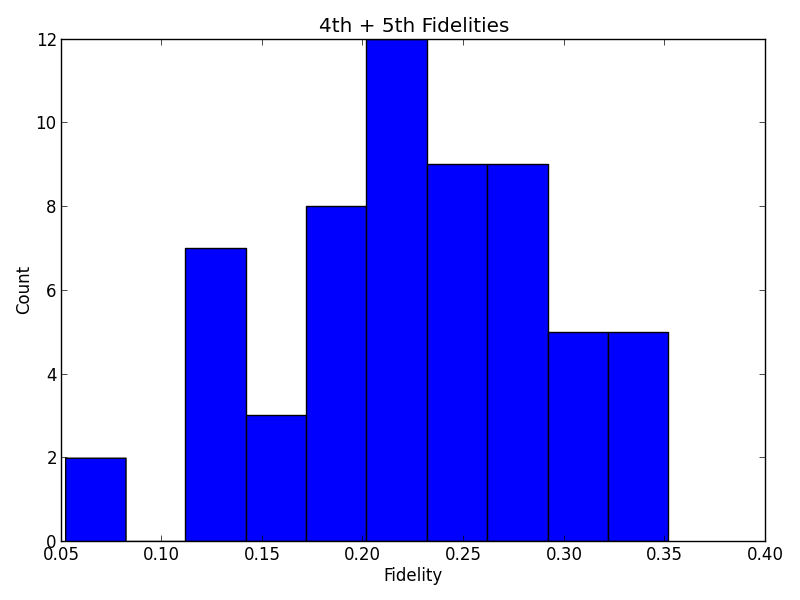
\includegraphics[bb= 0 0 800 600]{img/4_5_hist.png}
	}
	\caption[Short Time Fidelity Histogram]{Histogram of the fidelities found for all annealing times  $< 500 \mu$s.  Notice the gaussian like structure.}
	\label{fig:fid_hist}
\end{figure}

